
%......................................................................
\subsection{Automata}\label{sec:automata}

Automata are an appropriate means for describing \emph{time-dependent} systems, as
opposed to rules and facts that provide a \emph{static} view.

In the present form, the L4 automata are inspired by the theory of Timed
Automata \cite{larsen1997uppaal} and in particular by the Uppaal
systen\footnote{\url{https://uppaal.org/}}. Our long-term aim is to go beyond the model
checking capabilities of Uppaal by a mapping of automata to SMT solvers. As
long as this feature is under development, we try to achieve maximal
compatibility so that Uppaal can be used together with L4, in two directions:

\begin{itemize}
\item The internal L4 data structures can be printed in the Uppaal
  \texttt{*.xta} format. An example is given in \figref{fig:system_uppaal}.
\item \texttt{*.xta} files written by Uppaal can be read by L4, with minor
  syntactic differences and restrictions. An example is given in \figref{fig:system_l4}.
\end{itemize}
The above automata are graphically displayed in \figref{fig:uppaal_automaton}.

\begin{figure}
\centering
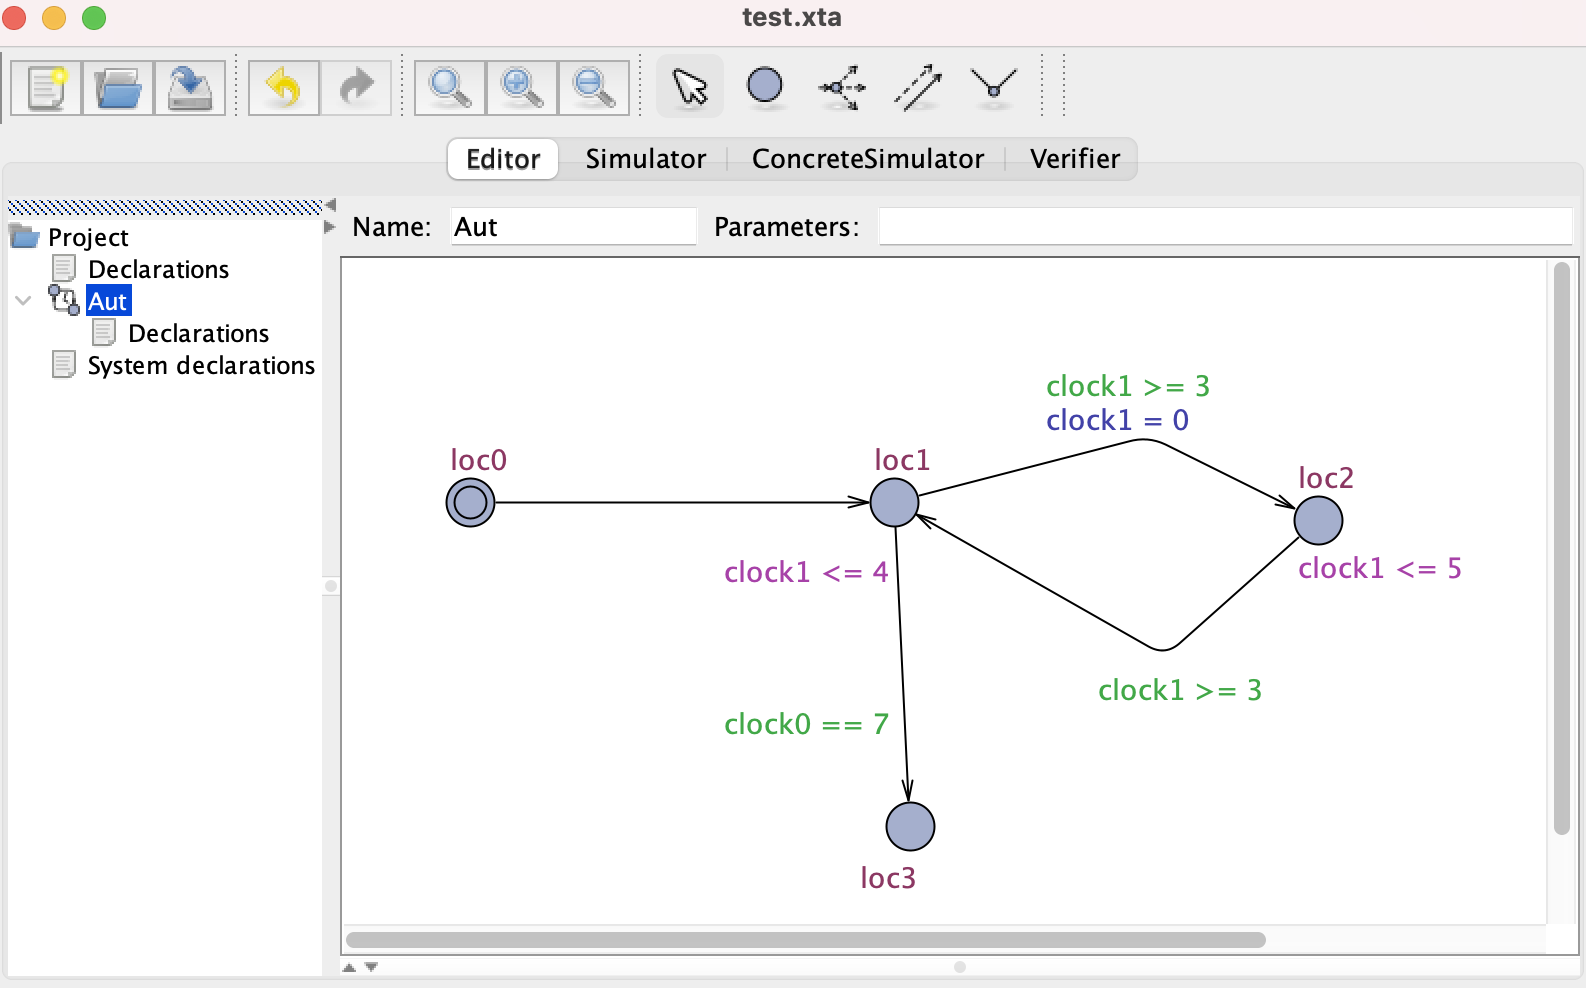
\includegraphics[scale=0.4]{Figures/uppaal_automaton.png}
\caption{Automaton represented in Uppaal}\label{fig:uppaal_automaton}
\end{figure}


These two methods will be revisited in the following.

\begin{figure}
  \begin{lstlisting}
chan x, y;
process Aut () {
    clock clock0, clock1;
    state
        loc0,
        loc1 { clock1 <= 4 },
        loc2 { clock1 <= 5 },
        loc3
        ;

    init loc0;
    trans
        loc1 -> loc3 { guard clock0 == 7 ;   },
        loc2 -> loc1 { guard clock1 >= 3 ;   },
        loc1 -> loc2 { guard clock1 >= 3 ;  assign clock1 = 0; },
        loc0 -> loc1 {    }
        ;
    }
system Aut; 
  \end{lstlisting}
  \caption{System specification in Uppaal format}\label{fig:system_uppaal}
\end{figure}

\begin{figure}
  \begin{lstlisting}
system AutSys {
    chan x, y;
    process Aut () {
        clock clock0, clock1;
        state
            loc0,
            loc1 { clock1 <= 4 },
            loc2 { clock1 <= 5 },
            loc3
            ;

        init loc0;
        trans
            loc1 -> loc3 { guard clock0 == 7 ;   },
            loc2 -> loc1 { guard clock1 >= 3 ;   },
            loc1 -> loc2 { guard clock1 >= 3 ;  assign clock1 = 0; },
            loc0 -> loc1 {    }
            ;
        }
    }
  \end{lstlisting}
  \caption{System specification in L4 format}\label{fig:system_l4}
\end{figure}



\subsubsection{Automata and Systems}

An \emph{automaton} is a graph commposed of nodes (states) and arcs
(transitions). States and transitions can be annotated with conditions
(temporal or not) and synchronization information. A \emph{system} is composed
of one or several automata and may contain declarations of channels (for
synchronization), clocks etc.


\subsubsection{From L4 to Uppaal}

The Uppaal \texttt{*.xta} format contains all the relevant structural
information for processing an automaton in Uppaal. However, no graphical
information is available, which typically leads to a poor layout when opening
an \texttt{*.xta} file.

An L4 program containing a system can be printed in Uppaal syntax with the
fake assertion
\begin{lstlisting}
  assert {printUp} True
\end{lstlisting}
which can be run as described in \secref{sec:running_solver}. The resulting
text can be written on a \texttt{*.xta} file and be processed by Uppaal. The
directive \texttt{printL4} produces the L4 format of automata.

Genuine proof obligations are currently not written to Uppaal (they would have
to be written to the corresponding \texttt{*.q} file).

\subsubsection{From Uppaal to L4}

A Uppaal \texttt{*.xta} file can be copied into L4 and then be manipulated as
any other L4 source. The L4 syntax and Uppaal syntax are sufficiently similar
so as to not require major changes, but the following manual postprocessing is
necessary:
\begin{itemize}
\item Automata and declarations belonging to one system have to be included
  into a system specification \texttt{system SysName \{ ... \}} as in
  \figref{fig:system_l4}. Several system specifications may coexist in an L4
  file.
\item Comments begin with a double slash (\texttt{//}) in Uppaal, which is not
  recognized by the L4 parser, and therefore have to be replaced by a sharp
  (\texttt{\#}) in L4.
\item Some expressions may be written differently, in particular the constants
  \texttt{True} and \texttt{False} which are written lowercase in Uppaal.
\end{itemize}

A notable difference is that Uppaal permits the declaration of automaton
\emph{templates} that can be instantiated. This is currently not possible in L4.



\remms[inline]{BEGIN TODO}
Note: there is another TODO file elsewhere. Integrate in this document, in a separate file to be excluded from compilation for the general public.
\begin{itemize}
\item local variable declarations not printed
\end{itemize}

\remms[inline]{END TODO}



%......................................................................
\subsection{Rules}\label{sec:rules}


%......................................................................
\subsection{SMT Solver}\label{sec:smt_solver}


\subsubsection{Assertions}\label{sec:assertions}


\subsubsection{Running the solver}\label{sec:running_solver}



%......................................................................
\subsection{Expert Systems}\label{sec:epert_systems}
\parskip=5pt plus 7pt
\parindent=15pt

Expert Systems are a way of replicating the logical reasoning and domain 
capabilities of a human expert through explicit knowledge capture.

L4 targets the use of expert systems as formal advisory interpreters; that form 
high-level conclusions given a set of ground truths and the application of formal 
axioms. 
\remal{There exists case-based legal expert systems, but my personal opinion is that these are less intuitive and much harder to support} 
Legal texts are typically well-structured \& formal, with well-defined 
terms integrated in clear and specific domains. However, there might be 
situations where the interpretive ability of a trained lawyer are required, 
but cannot be accessed due to the insufficient time or resources. Situations like
these are prime areas that expert systems excel in. Unfortunately,  
previous attempts at legal-specific expert systems in the 1980s and 1990s were 
largely exploratory and descriptive in nature, with no attempts at public testing. \cite{leith2016riseandfall}

In the time since, there have been various efforts into the building of rigorous 
and efficient rule-based systems.
\remal{To cite drool's rete, find clara's paper (if it exists) etc.} 
To build on the results of these efforts, we offer L4 as an upstream format that 
transpiles to such existing formats. 

As with existing expert systems, L4 files already mimic the characteristics 
of an easily modifiable knowledge base. 
Furthermore, this approach allows you, the user-developer/knowledge engineer, 
the option of choosing the language environment you would like to work with, and the 
flexibility of desigining a frontend user interface that would fit your purposes.

The currently supported rule-engine output formats are 
\href{https://docs.jboss.org/drools/release/7.58.0.Final/drools-docs/html_single/}{Drools} 
and 
\href{http://www.clara-rules.org/}{Clara-Rules}.



%%% Local Variables:
%%% mode: latex
%%% TeX-master: "main"
%%% End:
